\documentclass[12pt]{article}
\usepackage[a4paper, margin=.30in]{geometry}
\usepackage{graphicx ,
            wrapfig,
            xcolor, 
            enumerate,
            amsmath,fontenc,makecell,chemfig, multirow
            }
\usepackage{mhchem} 

\newcommand\headerMe[2]{\noindent{}#1\hfill#2}
\renewcommand{\thesection}{\Roman{section}}

%\title{Leçon N 6 : Le mouvement}
\author{Zakaria HAOUZAN}
\date{\today}

\begin{document}
% headers --------------
\headerMe{Matière : Physique-Chimie}{Professeur : Zakaria HAOUZAN}\\
\headerMe{Unité : Travail Mécanique et Energie }{Établissement : Lycée SKHOR qualifiant}\\
\headerMe{Niveau : TCS}{Heure : 4H}\\

% ------Content ________
\begin{center}

    \Large{Leçon $N^{\circ} 4 $: \color{red} La concentration molaire }
\end{center}

%\begin{wrapfigure}[10]{r}{0.5\textwidth}
%    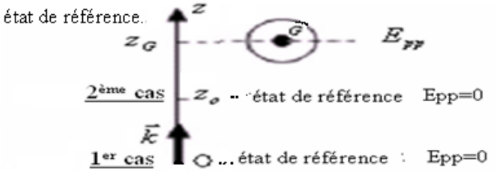
\includegraphics[width=0.5\textwidth]{./img/img00.png}
%\end{wrapfigure}

\section{Solution aqueuse et concentration molaire: }
\subsection{Solution aqueuse: }
\subsubsection{Notion de solution:}
Une solution est un mélange homogène obtenue par dissolution d'une espèce chimique dans un liquide appelé
solvant , (l'espèce chimique dissoute est appelée soluté).

donc Solvant + soluté $\ce{ -> }$ solution
\\le soluté : peut être solide , liquide ou gazeux .
\\le solvant : peut être soit : l'eau ou un liquide organique (comme l'alcool , le cyclohexane....)
\subsubsection{Solution aqueuse:}
Lorsqu'on prépare une solution en utilisant l'eau comme soluté, la solution obtenue est appelée solution aqueuse.
donc $\ce{Solvant + eau -> solution aqueuse}$

\subsection{Concentration molaire: }
La concentration molaire d'une espèce chimique en solution est égale à la quantité de matière de cette espèce
présente dans 1 litre de solution.
Elle est donnée par la relation suivante: $c = \frac{n}{V}$
\\n : la quantité de matière de l'espèce chimique X;
\\V le volume de la solution en (L)
\\c la concentration molaire en mol/L

Remarque: On peut déterminer la concentration d'une espèce chimique x dissoute dans un volume V à partir de
sa masse
\section{Dilution d'une solution: }
\subsection{Définition: }
La dilution d'une solution est un procédé qui consiste à obtenir une solution finale de concentration inférieure à
celle de la solution de départ tout en conservant la quantité de matière du soluté.

Donc la dilution d'une solution entraine la diminution de sa concentration

Pour diluer une solution initiale (solution mère) , on ajoute une quantité d'eau à un volume précis de la solution
mère . La solution obtenue par dilution est appelée solution fille (ou solution diluée).
\begin{wrapfigure}[5]{r}{0.4\textwidth}
  \begin{center}
    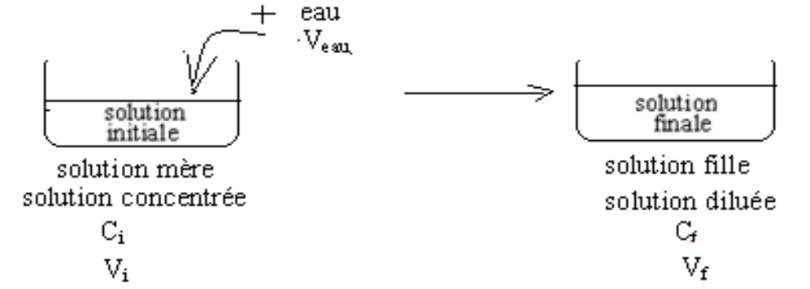
\includegraphics[width=0.39\textwidth]{./img/dilution_fig00.png}
  \end{center}
\end{wrapfigure}
\subsection{Relation de dilution:}
Généralement la solution diluée est obtenue par addition d'un certain volume d'eau à la solution mère.

Soit Ci la concentration de la solution initiale (solution mère) et Vi son volume. 

et Cf la concentration de la solution finale (solution fille) et Vf son volume. $V_f = V_i + V_{eau}$

Au cours de la dilution le volume augmente , la concentration diminue mais  la quantité de matière ne change pas Donc $n_i = n_f$

alors $C_i.V_i = C_f.V_f$ Cette relation est appelée relation de la dilution .

On définie le facteur de dilution par la relation : $F = \frac{C_i}{C_f} =\frac{V_f}{V_i}$

Par Exemple F = 10 On dit que la solution diluée 10 fois  
\section{Mode opératoire : préparation et dilution d'une solution:}
\subsection{Problématique:}
On veut préparer 100mL d'une solution de Chlorure de sodium de concentration C=1mol/L puis par dilution de
10mL de cette solution (de la solution préparée) on veut obtenir une solution de concentration C'= 0,01mol/L .
On donne :$M(N_a) = 23 g/mol et M(Cl) =35g/mol$

\begin{wrapfigure}{r}{0.1\textwidth}
  \begin{center}
    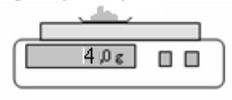
\includegraphics[width=0.1\textwidth]{./img/balance.png}
  \end{center}
\end{wrapfigure}
\subsection{1ère étape :Préparation de la solution: }
calculons tout d'abord la masse d'hydroxyde de sodium NaOH solide qu'on doit dissoudre dans un litre d'eau
distillée . : $m = C.M.V$ donc $C = \frac{n}{V} = \frac{m}{M.V}$
m = 1x58x0.1 = 5.8g

On mesure à l'aide d'une balance électronique 5.8g de chlorure de sodium NaCl solide

Puis on introduit l'introduit dans une fiole jaugée de 100mL et ensuite on ajoute de l'eau distillée jusqu'au trait de la jauge de la fiole et on agite jusqu'à la dissolution complète .
\begin{center}
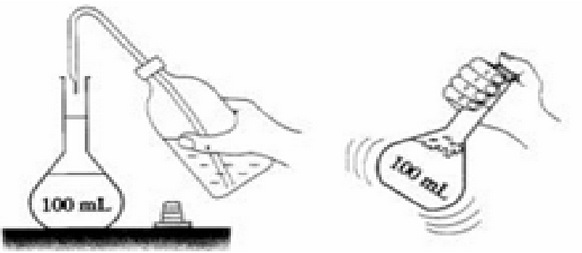
\includegraphics[width=0.4\textwidth]{./img/dilution_steps.png}
\end{center}
On obtient alors 100mL d'une solution de Chlorure de
sodium de concentration=1mol/L.

\subsection{2ère étape :dilution de la solution:}
Après avoir préparé la solution 1mol/L de Chlorure de sodium , on doit tout d'abord s'avoir le volume de la solution
mère qu'on doit diluer.
 
En effet : le coefficient de la dilution est:  $F = \frac{C}{C'} = 100$

On prélève donc un volume V=10mL de la solution mère de concentration C=1mol//L et par dilution on veut
obtenir une solution de volume V'=1L de concentration C'= 0,01mol/L.
donc V'=V+Veau d’où Veau=V'-V=1000-10=990mL.

On verse donc les 10mL de la solution mère dans une fiole jaugée de 1L et on complète avec l'eau distillée jusqu'au trait de la jauge.
\begin{center}
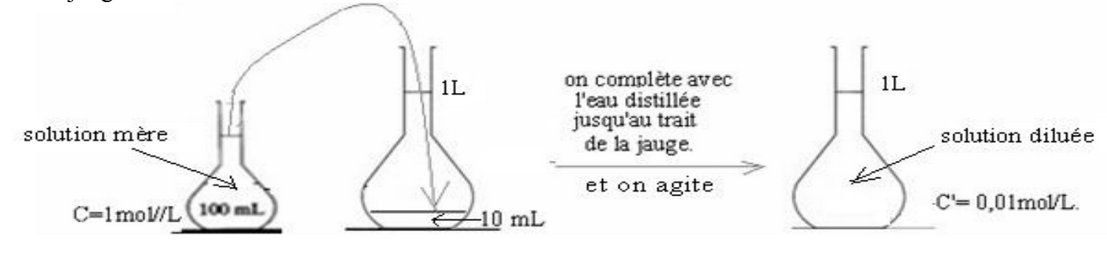
\includegraphics[width=0.9\textwidth]{./img/facteur_dilution.png}
\end{center}
\end{document}

